\section{Statik}
		
	\subsection{Schwerkraft (Gewichtskraft)}
	
		$$ \boxed{ \text{Allgemein:} \quad F_G = G \cdot \frac{m_1 \cdot m_2}{r^2} }$$
		$$ \boxed{ \text{Erde:} \quad  F_G = G \cdot \frac{m_E \cdot m}{r_E^2} = m \cdot g }$$ 
		
		\begin{tabular}{clc}
			$F_G$ & Gewichtskraft         & $[F_G] = \mathrm{\frac{kg \, m}{s^2} = N}$ \\
			$G$   & Gravitationskonstante & $6.67 \cdot 10^{-11} \mathrm{\frac{m^3}{kg \, s^2}}$ \\ 
			$m_i$ & Massen der Körper     & $[m] = \mathrm{kg}$ \\
			$r$   & Abstand der Massen    & $[r] =\mathrm{m}$ \\
			$g$   & Erdbeschleunigung     & $9.81 \mathrm{\frac{m}{s^2}}$ \\
			$m_E$ & Masse der Erde        & $5.972 \cdot 10^{24} \, \mathrm{kg} $ \\
			$r_E$ & Erdradius             & $6.378 \cdot 10^6 \, \mathrm{m}$ \\
		\end{tabular}
		
	\subsection{Normalkraft (Kontaktkraft)}
		(Sekundär-) Kraft, welche sich so anpasst, dass in Ruhe ein Kräftegleichgewicht herrscht: \\
		\\
		$\boxed{ F_G = -F_N}$ \qquad $\Rightarrow$ im Gleichgewicht auf horizontaler Oberfläche
				
	\subsection{Zerlegung von Kräften}
		Kraftvektoren kann man komponentenweise aufteilen: \\
		\\
		\begin{minipage}{0.6\linewidth}
			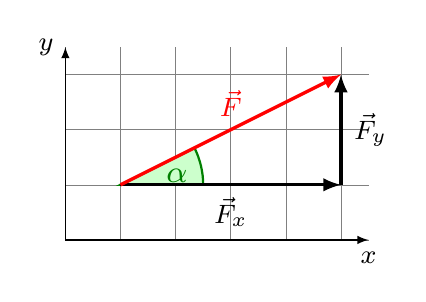
\begin{tikzpicture}
				[
				x=1cm, y=1cm, scale=0.7, font=\footnotesize, >=latex 
				%Voreinstellung für Pfeilspitzen
				]
				
				%Raster im Hintergrund
				\draw[step=1, gray, very thin] (0,0) grid (5.5,3.5);
				
				%Länge x Achse
				\draw [-latex] (0,0) -- ++(5.5,0) node[below, scale=1.2] {$x$};
				
				%Länge y Achse
				\draw [-latex] (0,0) -- ++(0,3.5) node[left, scale=1.2] {$y$};
				
				%Winkel
				\filldraw[fill=green!20!white, draw=green!50!black, thick] (1,1) -- (2.5,1) arc (0:26.56:1.5) -- cycle node[midway, below, green!50!black, scale=1.4, yshift=3pt, xshift=5pt] {$\alpha$};		
				
				%Vektor a
				\draw[-latex, very thick] (5,1) -- (5,3) node [midway, right, scale=1.2] {$\vec{F}_y$} node (Fy) {}; 
				%Vektor b
				\draw[-latex, very thick] (1,1) -- (5,1) node [midway, below, scale=1.2] {$\vec{F}_x$} node (Fx) {};

				%\draw[dashed] (a.center) -- ++ (3,0) node (c) {};
				%\draw[dashed] (b.center) -- ++ (2,3);
				\draw[very thick, red, -latex] (1,1) -- (Fy.center) node [midway, above, scale=1.2] {$\vec{F}$} node (F) {};
			\end{tikzpicture}
		\end{minipage}
		\hfill
		\begin{minipage}{0.6\linewidth}
			$\vec{F} = \vec{F}_x + \vec{F}_y + \vec{F}_Z$ \\	
			\\
			\textbf{hilfreich beim Lösen \\
			von Aufgaben!} \\
		\end{minipage}
		
	\subsection{Gleichgewichtsbedingungen für Massepunkte}
		Der Massepunkt erfährt keine Beschleunigung \\
		$\Rightarrow$ Summe aller wirkenden Kräfte ist 0 
		
		$$ \boxed{ \vec{R} = \sum \limits_{i = 1}^n \vec{F}_i = \vec{0} \qquad \Rightarrow \text{komponentenweise} }$$
		
		$$ \boxed{ \sum \limits_{i = 1}^n \vec{F}_x = \vec{0}  \qquad  \sum \limits_{i = 1}^n \vec{F}_y = \vec{0}  \qquad  \sum \limits_{i = 1}^n \vec{F}_z = \vec{0} } $$ 
			
	\subsection{Haftreibung / Gleitreibung}
	
		\subsubsection{Trockene Festkörperreibung}
	
			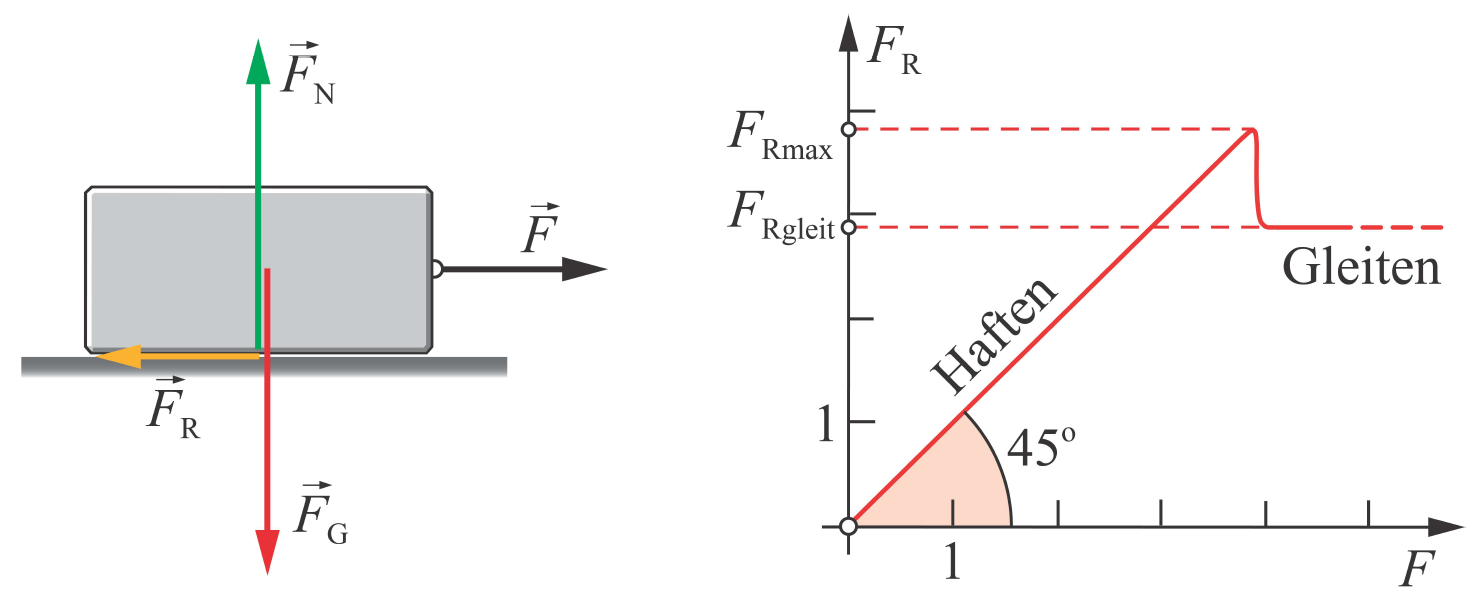
\includegraphics[width=0.7\linewidth]{Bilder/reibung} \\
		
			\begin{minipage}{0.65\linewidth}
				$$ \boxed{ \text{Haftreibung:} \quad \vec{F}_{R,max} = \mu_H \cdot \vec{F}_N } $$ 
				
				$$ \boxed{ \text{Gleitreibung:} \quad \vec{F}_{Gleit} \approx \mu_G \cdot \vec{F}_N } $$
			\end{minipage}
			\hfill
			\begin{minipage}{0.3\linewidth}
				$$ \boxed{ \vert \vec{F}_R \vert \leq \vert \vec{F}_{R,max} \vert } $$ \\
			\end{minipage}
		
			\begin{tabular}{lll}
				$\vec{F}_R$ & Reibungskraft & $[\vec{F}_R] = \mathrm{N}$ \\
				$\vec{F}_{R,max}$ & Haftreibungskraft & $[\vec{F}_{R,max}] = \mathrm{N}$ \\
				$\vec{F}_{Gleit}$ & Gleitreibungskraft & $[\vec{F}_{Gleit}] = \mathrm{N}$ \\
			\end{tabular}

		\subsubsection{Viskose Reibung}
			Sobald Schmiermittel zum Einsatz kommen, ist die Reibungskraft abhängig von der Grösse der Berührungsfläche: \\
			\\
			Bei gleicher Normalkraft $\vec{F}_N$ ist bei 
			
			\begin{tabular}{ll}
				$\bullet$ & kleinerem Flächendruck die Reibung kleiner \\
				$\bullet$ & grösserem Flächendruck die Reibung grösser \\
			\end{tabular}
		
	\subsection{Starre Körper}
	
		\begin{tabular}{ll}
			$\bullet$ & Ein starrer Körper wird durch angreifende Kräfte \\
			& nicht deformiert \\
			$\bullet$ & Bei einem starren Körper kann die Kraft entlang ihrer  \\
			& Wirkungslinie \underline{beliebig} verschoben werden \\
		\end{tabular}
	
	\subsection{Addition von Kräften}
		
		\subsubsection{Spezialfall: Ebene Kräftegruppe für schiefe Wirkungslinie}
			Kräfte entlang ihrer Wikungslinie verschieben \\
			$\Rightarrow$ Im Schnittpunkt vektorielle Addition der Kräfte durchführen, um die resultierende Kraft zu erhalten. \\
			\\
			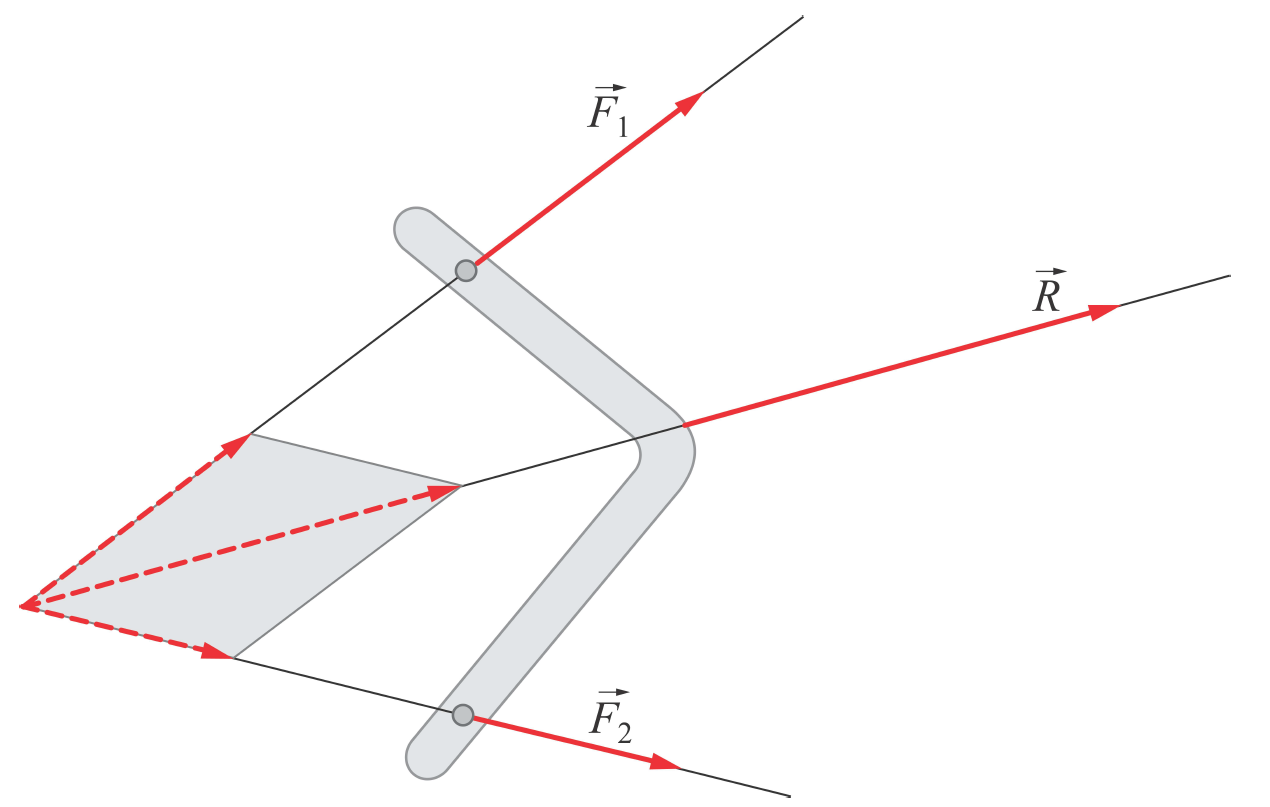
\includegraphics[width=0.7\linewidth]{Bilder/schneidende_wirkungslinien} \\
			\\
			Dieses Verfahren kann auch mehrfach angewendet werden!

		\subsubsection{Spezialfall: Ebene Kräftegruppe für parallele Wirkungslinie}
			Zwei sich zu null addierende Hilfskräfte hinzufügen ($\vec{H}_1 \; , \; \vec{H}_2$) \\
			\\	
			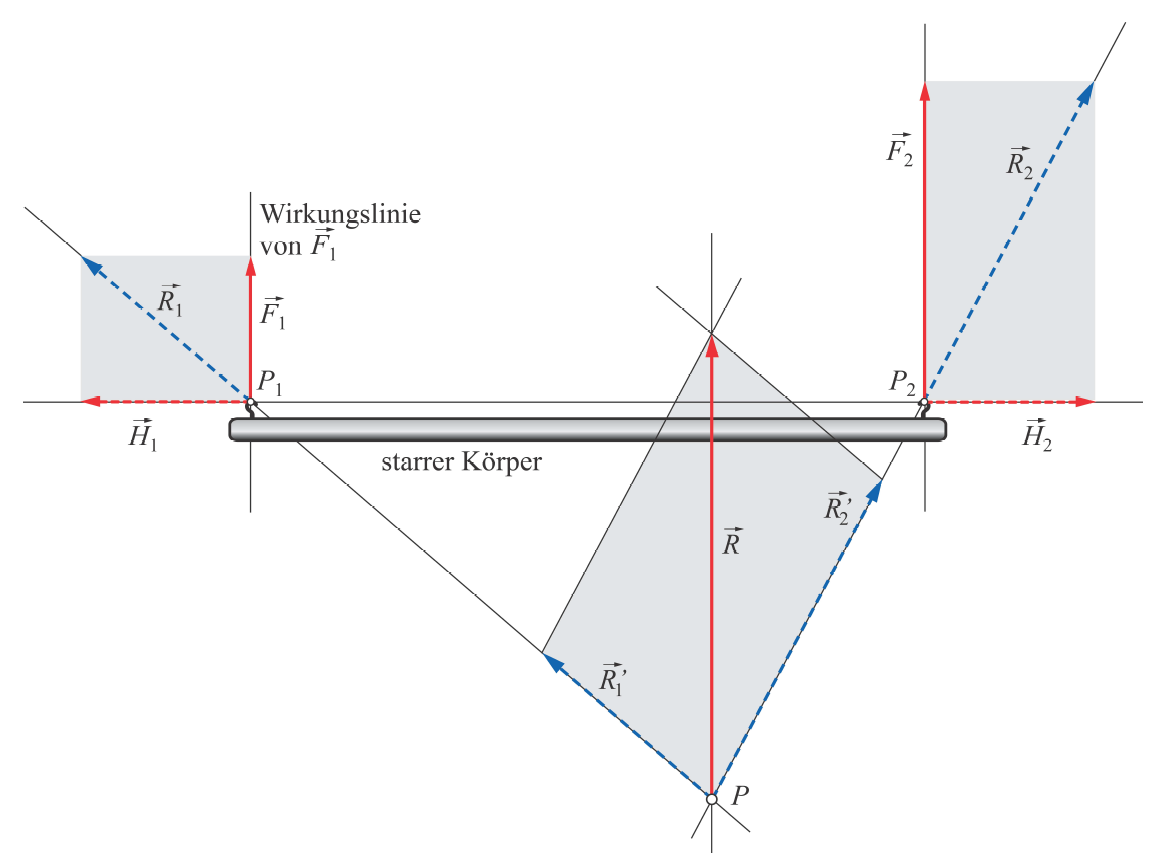
\includegraphics[width=0.7\linewidth]{Bilder/parallele_wirkungslinien}

		\subsubsection{Spezialfall: Ebene Kräftegruppe für parallel, entgegengesetzt und gleich grosse Kräfte}
	
			Kräftepaare können in andere Kräftepaare umgewandelt  werden, aber \underline{niemals zu einer} resultierenden Kraft $\vec{R}$ vereinfacht werden. \\
			\\
			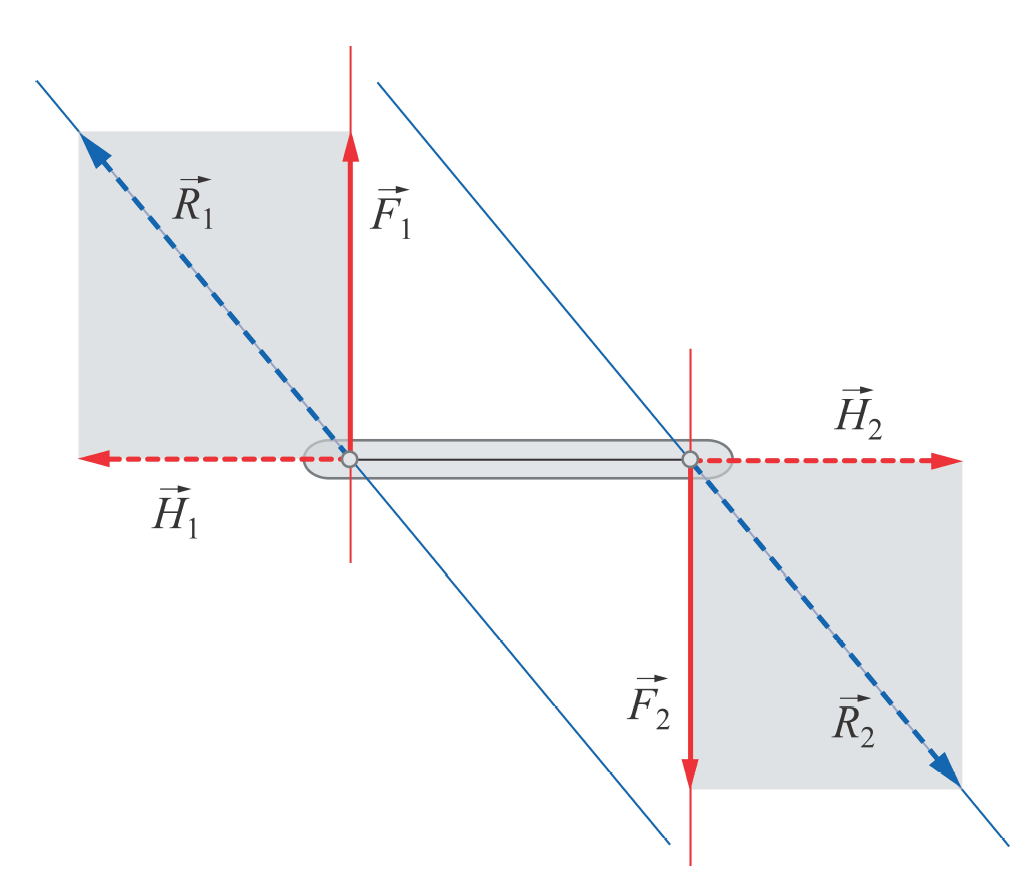
\includegraphics[width=0.7\linewidth]{Bilder/kraeftepaar_wirkungslinien}
		
	\subsection{Drehmoment}
		Eine Drehwirkung auf einen starren Körper lässt sich auf zwei \\
		verschiedene Arten und Weisen erzeugen: \\
		\\
		\begin{tabular}{ll}
			$\bullet$ & Kräftepaar \\
			$\bullet$ & einzelne Kraft und Bezugspunkt (Drehzentrum) \\
		\end{tabular}
		
		\begin{minipage}{0.48\linewidth}
			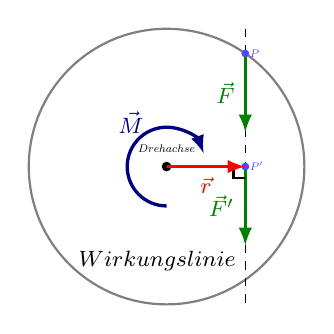
\begin{tikzpicture}
				[
				x=1cm, y=1cm, scale=0.5, font=\footnotesize, >=latex 
				%Voreinstellung für Pfeilspitzen
				]
				%Raster im Hintergrund
				%\draw[step=1, gray, very thin] (-5.5,-5.5) grid (5.5,5.5);
				\draw[thick, gray] (0, 0) circle(3.5);
				\draw[dashed] (2,3.5) -- (2,-3.5) node [midway, left, yshift=-1.2cm] {$Wirkungslinie$};
				\draw[-latex, draw=blue!50!black, very thick, rotate = -90] (1,0)--(1,0) arc(0:-250:1) 
								node [midway, above, xshift=-1.3pt, yshift=0, blue!50!black] {$\vec{M}$} {};
				\fill[black] (0, 0) circle(3.5pt) node [midway, above, yshift=7pt] {$Drehachse$};
				\begin{scope}[xshift=2cm, yshift=0cm, rotate=0, scale=1]
					%Kräfte
					\draw [-latex, very thick, green!50!black] (0,0) -- ++(0,-2) node[midway, left] {$\vec{F}{'}$};
					\fill [blue!70!white](0,0) circle (0.1) node[midway, right] {$P'$};;
				\end{scope}		
				\begin{scope}[xshift=2cm, yshift=0cm, rotate=90, scale=1]  		
					\draw [thick](-0.3,0) -- (-0.3,0.3) -- (0,0.3);
				\end{scope}	
				\begin{scope}[xshift=2cm, yshift=2.87228cm, rotate=0, scale=1]
					%Kräfte
					\draw [-latex, very thick, green!50!black] (0,0) -- ++(0,-2) node[midway, left] {$\vec{F}$};
					\fill [blue!70!white](0,0) circle (0.1) node[midway, right] {$P$};;
				\end{scope}	
				\draw[-latex, very thick, red] (0,0) -- ++(2,0) node[midway, below] {$\vec{r}$};
			\end{tikzpicture}
			\\
		\end{minipage}
		\hfill
		\begin{minipage}{0.48\linewidth}
			$ \vert \vec{M} \vert = \vert \vec{r} \times \vec{F} \vert = a \cdot \vert \vec{F} \vert  $	\\
			\\
			Die Länge a muss \textbf{senkrecht} zur wirkenden Kraft sein!
		\end{minipage}

		\begin{tabular}{lll}
			$\vec{M}$ & Drehmoment & $[M] = \mathrm{Nm}$ \\
			$\vec{r}$ & Abstandsvektor & $[r] = \mathrm{m}$ \\
			$\vec{F}$ & Angreifende Kraft & $[F] = \mathrm{N}$ \\
		\end{tabular}

	\subsection{Gleichgewichtsbedungungen für starre Körper}
		
		$ \sum \limits_{i = 1}^n \vec{F}_i = \vec{0}$  \qquad  $ \sum \limits_{i = 1}^m \vec{M}_i = \vec{0} $  \qquad $\Rightarrow$ komponentenweise
	
	\subsection{Gleichgewichts-Arten}	
		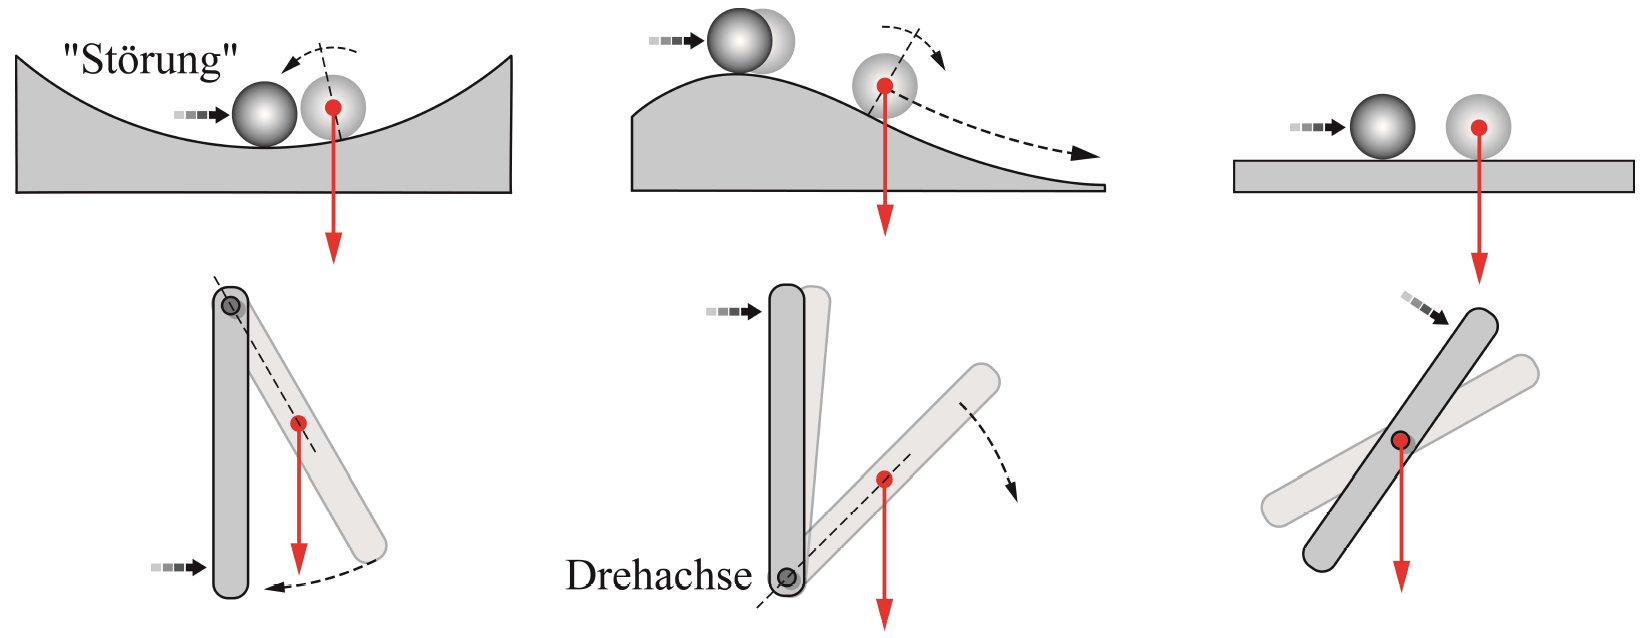
\includegraphics[width=0.95\linewidth]{Bilder/gleichgewichte} \\
		\\
		\begin{minipage}{0.3\linewidth}
			\center{stabil}
		\end{minipage}
		\hfill
		\begin{minipage}{0.3\linewidth}
			\center{labil}
		\end{minipage}
		\hfill
		\begin{minipage}{0.3\linewidth}
			\center{indifferent}
		\end{minipage}

	\subsection{Deformierbare Körper}
		
		\subsubsection{Spannungen}
			\textbf{Zugspannung $\sigma$} \\
				\\
				senkrecht wirkende Kraft pro Flächeneinheit \\
				Wenn $\sigma < 0$ spricht man von \textbf{Druck} 
				
				$$ \boxed{ \sigma = \frac{F_{\perp}}{A} } \qquad [\sigma] = \mathrm{\frac{N}{m^2}}$$ 

			\textbf{Schubspannung $\tau$ (Scherung)} \\
				\\
				parallel wirkende Kraft pro Flächeneinheit 
				
				$$ \boxed{ \tau = \frac{F_{\shortparallel}}{A} } \qquad [\tau] = \mathrm{\frac{N}{m^2}}$$

		\subsubsection{Dehnung $\epsilon$ (Hook'sches Gesetz)}
			$$ \boxed{ \epsilon = \frac{1}{E} \cdot \sigma = \frac{1}{E} \cdot \frac{F_{\perp}}{A} = \frac{\Delta \, l}{l} } $$ 

			\begin{tabular}{c l c}
				$\epsilon$ & Dehnung & $[\epsilon] = 1$ \\
				$E$ & Elastizitätsmodul (Materialeigenschaft) & $[E] = \mathrm{\frac{N}{m^2}}$ \\
				$l$ & Länge des Körpers vor Dehnung & $[l] = \mathrm{m}$ \\
				$\Delta \, l$ & Längenunterschied bei Dehnung & $[\Delta \, l] = \mathrm{m}$ \\
				$\sigma$ & Zugspannung & $[\sigma] = \mathrm{N}$ \\
				$A$ & Querschnittsfläche & $[A] = \mathrm{m^2}$ \\
				\\
			\end{tabular}
			
			$\Rightarrow$ \textbf{Das Hook'sche Gesetz gilt nur, solange die Deformation linear-elastisch ist!}

			%todo: Bild von Elastizität finden und einfügen

		\subsubsection{Querkontraktion $\epsilon_q$}
			Wird ein Stab gedehnt (länger), so wird er automatisch auch dünner \\		
			
			$$ \boxed{ \epsilon_q = \frac{\Delta \, d}{d} = - \mu \, \epsilon } \qquad \mu \in (0 \, ; \, 0.5)$$ \\
			
			\begin{tabular}{c l c}
				$\epsilon_q$ & Querkontraktion & $[\epsilon_q] = 1$ \\
				$d$ & Ursprüngliche Dicke des Materials & $[d] = \mathrm{m}$ \\
				$\Delta d$ & Dicken-Änderung & $[ \Delta \, d] = \mathrm{m}$ \\
				$\epsilon$ & (Längs-) Dehnung & $[\epsilon] = 1$ \\
				$\mu$ & Poisson-Zahl (Materialeigenschaft) & $[\mu] = 1$ \\
			\end{tabular}
		
		\subsubsection{Kompression $\frac{\Delta \, V}{V}$}
			Ein Körper wird von allen Seiten mit dem gleichen Druck belastet, sodass sich sein Volumen verkleinert 
			
			$$ \boxed{ \frac{\Delta \, V}{V} = - \kappa \cdot \Delta \, p } \qquad \Big( K = \frac{1}{\kappa} \Big) $$ \\ 
			
			\begin{tabular}{c l c}
				$V$ & Ursprüngliches Volumen des Körpers & $[V] = \mathrm{m^3}$ \\
				$\Delta V$ & Volumenänderung & $[\Delta V] = \mathrm{m^3}$ \\
				$\kappa$ & Kompressibilität & $[\kappa] = \mathrm{\frac{m^2}{N}}$ \\
				$\Delta \, p$ & Druckänderung & $[\Delta \, p] = \mathrm{\frac{N}{m^2} = Pa}$  \\ 
			\end{tabular}
			
			$$ \boxed{ \text{Würfel:} \quad \Rightarrow \kappa = \frac{3}{E} (1 - 2 \, \mu) }$$ 
			
			\textbf{Völlig inkompressibler Körper:} $\kappa = 0$  \qquad $K = \infty$ \qquad $\mu = 0.5$

		\subsubsection{Schubbeanspruchung (Scherung)}
		
			$$ \boxed{ \gamma = \frac{1}{G} \, \tau }$$ 
			
			$$ \boxed{ G = \frac{E}{2(1 + \mu)}  \quad \text{(gilt für isotrope Materialen)} } $$\\

			\begin{tabular}{c l c}
				$\gamma$ & Scherwinkel & $[\gamma] = \; ^\circ $ \\
				\rule{0pt}{10pt}$G$ & Schubmodul; Gleitmodul; Torsionsmodul & $[G] = \mathrm{\frac{N}{m^2}}$ \\
				\rule{0pt}{10pt}$\tau$ & Schubspannung & $[\tau] = \mathrm{\frac{N}{m^2}}$ \\
				\rule{0pt}{10pt}$E$ & Elastizitätsmodul (Materialeigenschaft) & $[E] = \mathrm{\frac{N}{m^2}}$ \\
				$\mu$ & Poisson-Zahl (Materialeigenschaft) & $[\mu] = 1$ \\
			\end{tabular}

		\subsubsection{Torsionsfeder}
		
			$$ \boxed{ M = c \cdot \varPhi \quad \quad c = \frac{\pi G r^4}{2l} }$$ 

			\begin{tabular}{c l c}
				$M$ & Drehmoment & $[M] = Nm$ \\
				$c$ & Auslenkkonstante & $[c] = $ \\
				$\varPhi$ & Auslenkwinkel & $[\varPhi] = \; ^\circ $ \\
				$G$ & Schubmodul & $[G] = \mathrm{\frac{N}{m^2}}$ \\
				$r$ & Radius der Feder & $[r] = m$ \\
				$l$ & Länge der Feder & $[l] = m$ \\
			\end{tabular}

		\subsubsection{Schraubenfeder}
		
			$$ \boxed{ F = c \cdot \Delta l \quad \quad c = \frac{G r^4}{4nR^3} }$$ 

			\begin{tabular}{c l c}
				$F$ & Kraft & $[F] = N$ \\
				$c$ & Auslenkkonstante & $[c] = $ \\
				$\Delta l$ & Längenänderung & $[\Delta l] = m$ \\
				$G$ & Schubmodul & $[G] = \mathrm{\frac{N}{m^2}}$ \\
				$r$ & Drahtradius der Feder & $[r] = m$ \\
				$R$ & Windungsradius der Feder & $[R] = m$ \\
				$n$ & Anzahl Windungen & $[n] = $ \\
			\end{tabular}

		\subsubsection{Blattfeder}
		
			$$ \boxed{ z = \frac{4l^3}{E \cdot b \cdot h^3}F }$$ 

			\begin{tabular}{c l c}
				$F$ & Kraft & $[F] = N$ \\
				$z$ & Verbiegung & $[z] = m$ \\
				$l$ & Längenänderung & $[l] = m$ \\
				$E$ & Elastizitätsmodul & $[E] = \mathrm{\frac{N}{m^2}}$ \\
				$b$ & Breite des Querschnitts & $[b] = m$ \\
				$h$ & Höhe des Querschnitts & $[h] = m$ \\
			\end{tabular}

	\subsection{Schiefe Ebene (mit Seil)}
		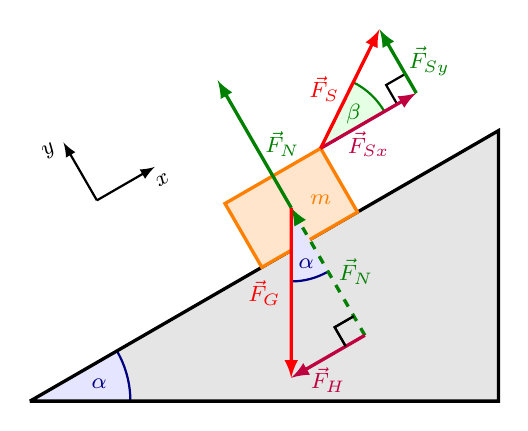
\begin{tikzpicture}
			[
			x=1cm, y=1cm, scale=0.85, font=\footnotesize, >=latex 
			%Voreinstellung für Pfeilspitzen
			]
			
			%Raster im Hintergrund
			%\draw[step=1, gray, very thin] (0,0) grid (7,6);	

			%Grunddreieck	
			\draw [fill=gray!20] (0,0) -- (7,0) -- (7,4.04145) -- (0,0);
			
			%Winkel
			\filldraw[fill=blue!10, draw=blue!50!black, thick] (0,0) -- (1.5,0) arc(0:30:1.5) 
				node [midway, xshift=-10pt, yshift=-3, blue!50!black] {$\alpha$} {};
					
			\draw [very thick] (0,0) -- (7,0) -- (7,4.04145) -- (0,0);
					
			%Bezugssystem
			\begin{scope}[xshift=1cm, yshift=3cm, rotate=30, scale=1]
				%Länge x Achse
				\draw [-latex, thick] (0,0) -- ++(1,0) node[below, rotate=30] {$x$};
			
				%Länge y Achse
				\draw [-latex, thick] (0,0) -- ++(0,1) node[left, rotate=30] {$y$};
			\end{scope}
			%Alles was gedreht wurde (Masse m, Kräftevektoren, ...)
			\begin{scope}[xshift=3.464cm, yshift=2cm, rotate=30, scale=1.1]

				\coordinate (A) at (0.75,0.5);
				\coordinate (B) at (0.75,-1.5);
				
				%Rechteck
				\draw [fill=orange!20!white] (0,0) rectangle (1.5,1);
				\draw [orange, very thick] (0,0) rectangle (1.5,1) node [midway, right, xshift=3pt, yshift=3pt] {$m$} {} ;
				
				%Vektoren Kraft-Seil
				\begin{scope}[xshift=1.5cm, yshift=1cm, rotate=0, scale=1]
					\begin{scope}[xshift=0cm, yshift=0cm, rotate=0, scale=1]
						\filldraw[fill=green!10, draw=green!50!black, thick] (0,0) -- (1,0) arc(0:33.6900:1) 
							node [midway, left, xshift=0pt, yshift=-7, green!50!black] {$\beta$} {};
					\end{scope}
					\coordinate (C) at (1.5,0);
					\coordinate (D) at (1.5,1);
					%Rechter Winkel
					\draw [thick](1.2,0) -- (1.2,0.3) -- (1.5,0.3);
					\draw [-latex, very thick, purple] (0,0) -- ++ (C) node [midway, below] {$\vec{F}_{Sx}$} {};
					\draw [-latex, very thick, green!50!black] (C) -- ++ (0,1) node [midway, right] {$\vec{F}_{Sy}$} {};
					\draw [-latex, very thick, red] (0,0) -- ++ (D) node [midway, left] {$\vec{F}_S$} {};
					%Rechter Winkel
				
				\end{scope}	
				
				%Vektoren FN, FG, FH
				
				\begin{scope}[xshift=0cm, yshift=0, rotate=0, scale=1]
					\coordinate (A) at (0.75,0.5);
					\coordinate (B) at (0.75,-1.5);
					\begin{scope}[xshift=0.75cm, yshift=0.5cm, rotate=-120, scale=1]
						\filldraw[fill=blue!10, draw=blue!50!black, thick] (0,0) -- (1,0) arc(0:30:1) 
							node [midway, above, xshift=-1.5pt, yshift=0, blue!50!black] {$\alpha$} {};
					\end{scope}
					%Rechter Winkel
					\draw [thick](0.45,-1.5) -- (0.45,-1.2) -- (0.75,-1.2);  
					\draw [-latex, very thick, dashed, green!50!black] (B) -- (A) node [midway, right] {$\vec{F}_N$} {};
					\draw [-latex, very thick, green!50!black] (A) -- ++(0,2) node [midway, right] {$\vec{F}_N$} {};
					\draw [-latex, very thick, purple] (B) -- ++(-1.1547,0) node [midway, below] {$\vec{F}_H$} {};
					\draw [-latex, very thick, red] (A) -- ++(-1.1547,-2) node [midway, left] {$\vec{F}_G$} {};
					%Rechter Winkel
					\draw [thick](0.45,-1.5) -- (0.45,-1.2) -- (0.75,-1.2);  
				\end{scope}		    		
			\end{scope}
			
		\end{tikzpicture}
		\\
		\textbf{Wichtige Formeln und Zusammenhänge zur schiefen Ebene} \\
			\\
			\begin{tabular}{lll}
				$F = m \cdot a$  & $F_G = m \cdot g$ \\
				\\
				$F_N = m \cdot g \cdot \cos(\alpha)$ & 
				$F_H = m \cdot g \cdot \sin(\alpha)$ \\
			\end{tabular}

	\subsection{Rezept: Aufgaben zur Statik lösen}
	
	\begin{tabular}{ll}
		1. & Koordinatensystem festlegen  \\
		2. & Alle wirkenden Kräfte einzeichnen \\
		3. & Bezugspunkt P (Drehpunkt) festlegen \\
		& $\Rightarrow$ \textbf{Da wo viele Kräfte} (oder da wo sinnvoll) \\
		4. & Kräfte komponentenweise aufschreiben: $\sum \vec{F}_i = 0$ \\
		5. & Drehmomente M aufschreiben und gleichsetzen: $\overleftarrow{M} = \overrightarrow{M}$ \\
	\end{tabular}

	\vfill\null
	\pagebreak
		